\section{Caratteristica Volt-Amperometrica di una lampadina}
Tratteremo ora l'analisi di un carico resistivo non ohmico. Per eseguire questa parte dell'esperienza abbiamo utilizzato una lampadina. Sappiamo che, quando abbiamo davanti una resistenza che si comporta in modo "ohmico", il grafico della caratteristica Volt-Amperometrica è una retta. Nel caso della lampadina, ci aspettiamo dunque una curva non lineare. Per poter apprezzare la forma di tale curva, abbiamo deciso di sottoporre il circuito (che non riportiamo in figura in quanto è identico a quello in $figura$ 1 e 2, con la sola differenza che al posto della resistenza vi è una lampadina) a vari valori di tensione, fino al valore massimo permesso dalle caratteristiche della lampadina. Riportiamo tali valori nel grafico seguente.

\begin{figure}[t]
    \centering
        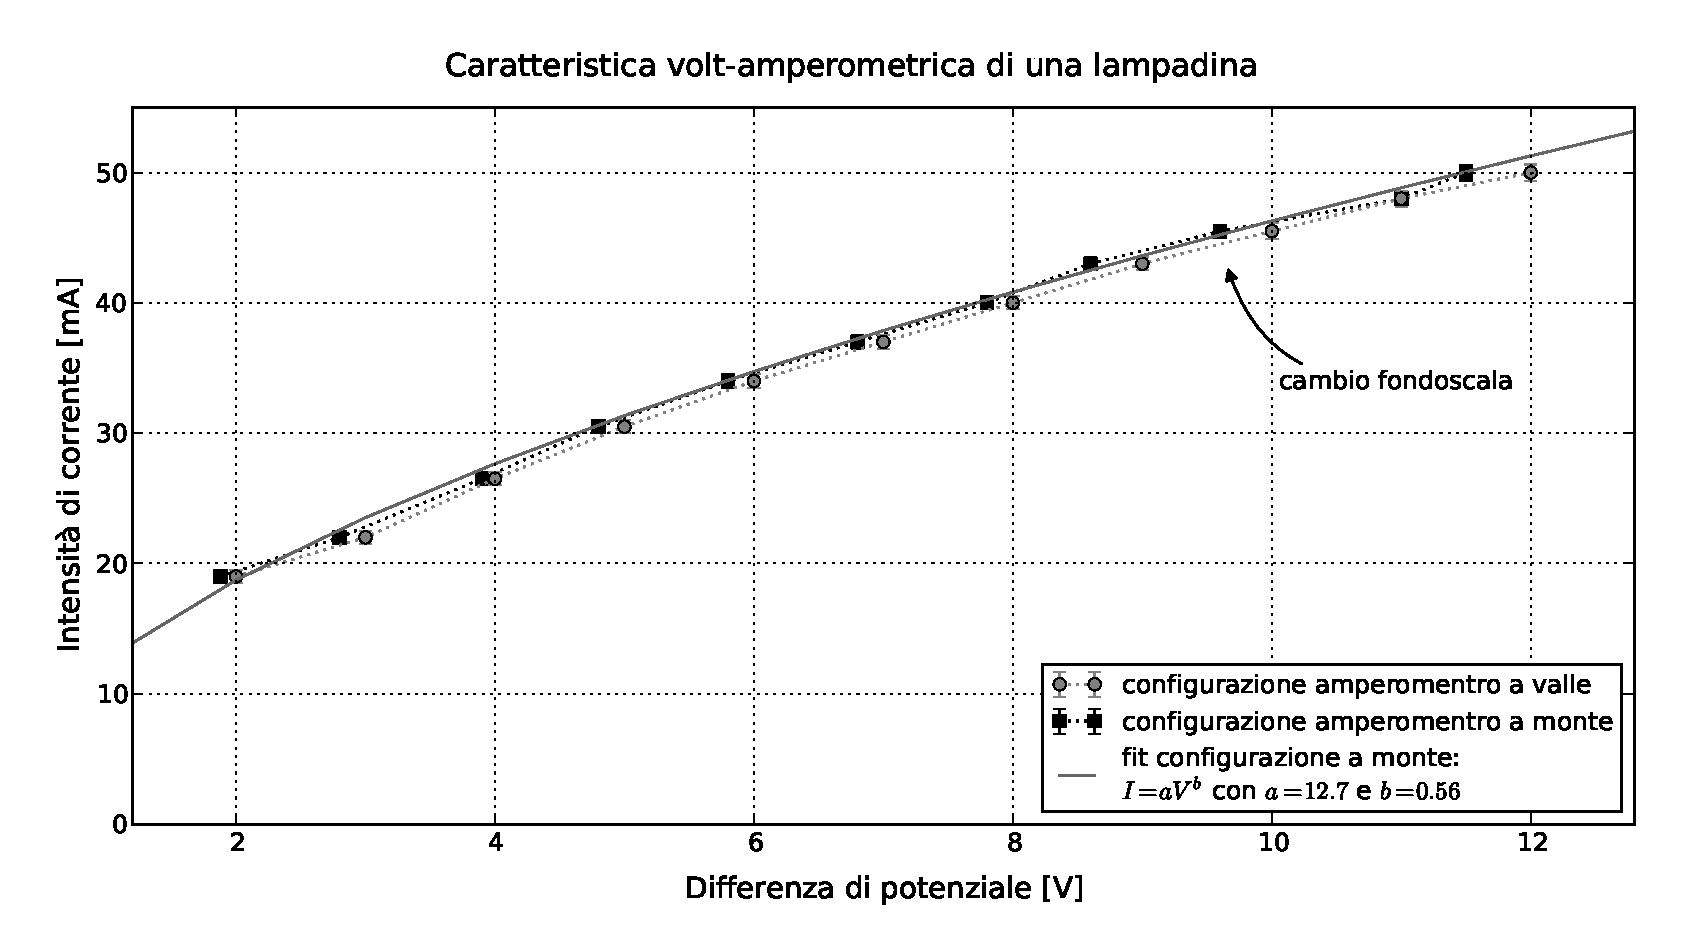
\includegraphics[width=\textwidth]{lamp.eps}
        \caption{Il grafico mostra la caratteristica volt-amperometrica di un carico resistivo non ohmico (lampadina).}
        \label{fig:lampadina}
\end{figure}